\section{On the sparsification choice for $\ell_1$ regularized problems}\label{sec:distributed-adaptive}

Assuming that all machines are responsive (i.e. $m\to \infty$ when $k\to\infty$), the inequality \eqref{eq:dif_prob} gives linear convergence of the mean squared error in terms of epochs if
\begin{equation}\label{eq:prob_gap}
    \frac{\pmin}{\pmax} > (1-\gamma \mu)^2 \stackrel{\gamma = \frac{2}{\mu + L}}{\geq} \left(\frac{1-\kappa_{\eqref{eq:pb}}}{1+\kappa_{\eqref{eq:pb}}}\right)^2
\end{equation}
and thus the behavior of the algorithm depends if the selection is performed uniformly (and thus structure-blind) or non-uniformly (to encompass some prior information).

\paragraph{Inefficiency of uniform sparsification}

If the selection is \emph{uniform}, i.e. if $p_i=\pp\in(0,1]$ for all $i$, $x^k\to x^\star$ in probability. Furthermore, the mean squared error vanishes linearly in terms of epochs with a rate $(1-\pp\gamma\mu(2-\gamma\mu))$. As a result, under the mild assumption over the delays (Assumption \ref{hyp:delident}) we could prove an almost sure convergence $\barx^k\to \barx^\star$ and as a corollary the identification property (see Theorem \ref{th:identification}) of \spy~with uniform sampling.

\begin{assumption}[Additional assumption for identification]
\label{hyp:delident}
The number of iterations between two full updates cannot grow exponentially, i.e. $k_{m+1}-k_m = o(\exp(m))$.
This assumption is rather mild and subsumes the usual bounded delay assumption.
\end{assumption}

This assumption, together with an exponential decrease in terms of mean squared error, implies the following result.

\begin{lemma}[Almost-sure convergence of \spy]\label{lm:spydr_identification}
Let the functions $(f_i)$ be $\mu$-strongly convex ($\mu>0$) and $L$-smooth and assumptions \ref{hyp:algo} and \ref{hyp:delident} hold. Select the probability vector $\pvec$ such that \eqref{eq:prob_gap} holds then $\barx^k$ converges almost surely to $\barx^k$.
\end{lemma}
\begin{proof}[Proof of Lemma \ref{lm:spydr_identification}]
Recall first from the end of the proof of Theorem~\ref{lm:spy_diff} that we have
for some $C$ and $\delta\in]0,1]$
\begin{equation}\label{eq:recall}
    \mathbb{E}\|\barx^k - \barx^\star\|^2 \leq C (1-\delta)^m.
\end{equation}
Notice that the exponent is not the iteration number but rather the number of stopping times $(k_m)$ before $k$. Thus, we can decompose the sum of the  
$( \|x^k - x^\star \|^2 )_k$ by epochs and get in expectation 
\begin{align*}
    \EE\left[ \sum_{k=1}^{+\infty}  \|\barx^k - \barx^\star \|^2 \right] 
    \leq \EE\left[ \sum_{m=1}^{+\infty} \sum_{k=k_m}^{k_{m+1}-1} \|\barx^k -\barx^\star \|^2 \right]
    \leq C \sum_{m=1}^{+\infty} (k_{m+1}-1 - k_m) (1-\delta)^m.
\end{align*}
Assumption~\ref{hyp:delident} now allows us to bound $k_{m+1}-1 - k_m$ and to get that this sum is finite almost surely:
\[
1 = \mathbb{P}\left[ \sum_{k=1}^{+\infty}  \|\barx^k - \barx^\star \|^2 < +\infty \right] \leq \mathbb{P}\left[ \|\barx^k - \barx^\star \|^2 \to 0 \right],
\]
which means that $(\barx^k)$ converges almost surely to $\barx^\star$.
\end{proof}

Almost sure convergence result guarantees the identification of the near-optimal support by iterates of the algorithms in the finite time (see Theorem \ref{th:identification}) with $u^k = \barx^k$ and \eqref{eq:s_to_supp}. 


Unfortunately, uniform selection usually results in poor performance in practice, as displayed in Figure~\ref{fig:uniform}. Hence the need for a more adaptive sparsification manner.

\begin{figure}[H]
\begin{center}
\subfloat[][The functional suboptimality versus the amount of iterations/gradient computations/communication rounds done.]{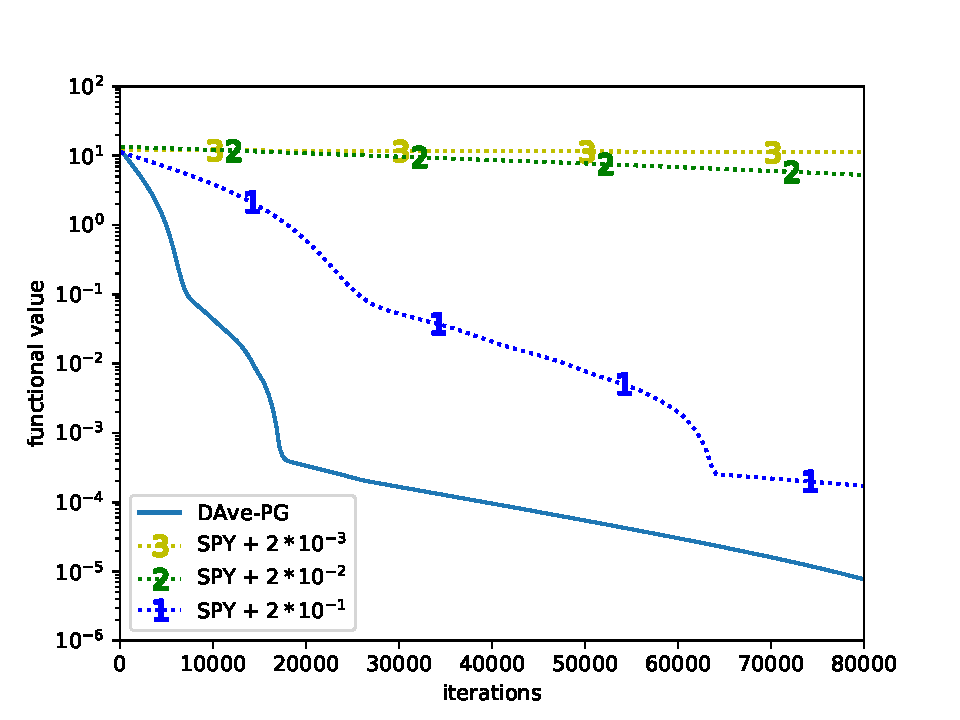
\includegraphics[width = 0.49\linewidth]{distributed/figs/madelon_10w_001_0001_fun_vs_ite_log_coordinate.pdf}}
 \hfill
\subfloat[][The functional suboptimality versus amount of coordinates sent during communication rounds.]{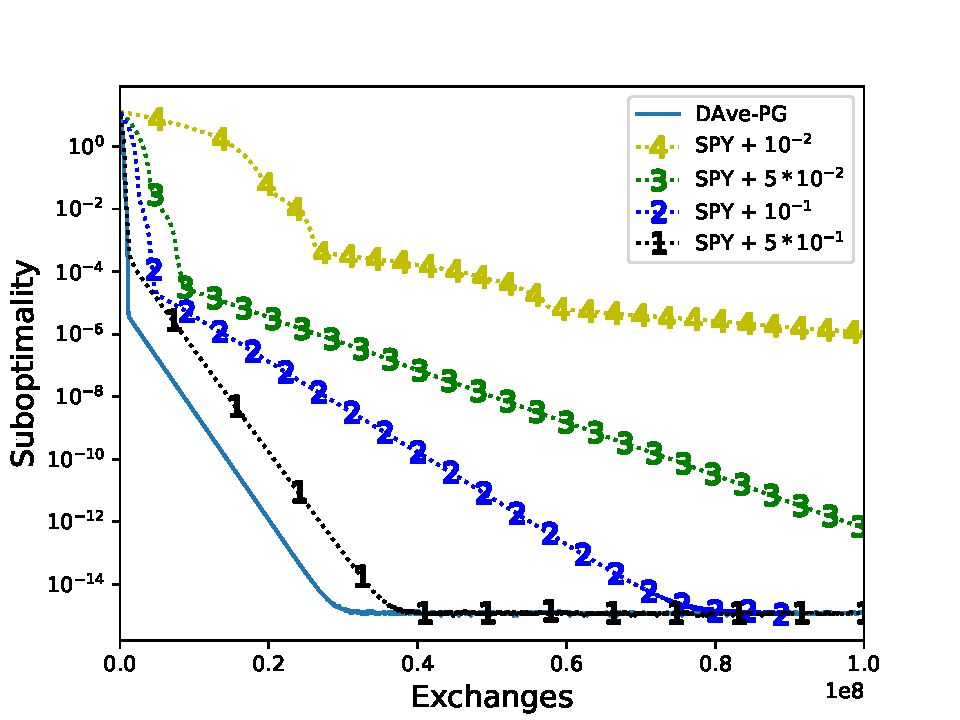
\includegraphics[width = 0.49\linewidth]{distributed/figs/madelon_10w_001_0001_fun_vs_ex_log_coordinate.pdf}}
\end{center}
\caption{Evolution of \salgo~iterates comparing to \dave. We consider logistic regression objective function with elastic net regularizer on Madelon dataset from LibSVM library \cite{chang2011libsvm}. We denote by ``SPY~+ $p$'' the \salgo with uniform probability $p$.}
\label{fig:uniform}
\end{figure}


\paragraph{Efficiency of adaptive sparsification}
\label{sec:adapt}

The idea of adaptively using the identified structure in coordinate descent for $\ell_1$-regularized problems methods was recently developed in \cite{grishchenko2020proximal} (see Section \ref{sec:mor-adaptive-subspace}. Mathematically, this means select coordinates in the mask as follows
\begin{assumption}[Sparsification with support identification]
\label{hyp:algoident}
The sparsity mask selectors $(\mathbf{S}^k)$ are random variables such that   $\mathbb{P}[j\in\mathbf{S}^k]=1$ if $j \in \supp({x^k})$ and either:
\begin{itemize}
    \item[] \textbf{\emph{Option I.}}
    $\mathbb{P}[j'\in\mathbf{S}^k] = \pi \in(0,1] $ for all $j'\!\notin \supp({x^k})$.
    \item[] \textbf{\emph{Option II.}}  $|\mathbf{S}^k| = |\supp({x^k})| + \pi(n - |\supp({x^k})|) \in \{ 1,..,n \} $ almost surely and  $\mathbb{P}[j'\in\mathbf{S}^k]=\mathbb{P}[j''\in\mathbf{S}^k]$ for all $j',j''\notin \supp({x^k})$.
\end{itemize}
% Furthermore, the delays $(D_i^k)_{i=1,..,M}$ are independent of the future mask selectors  $\{\mathbf{S}^\ell\}_{\ell\geq k}$.
\end{assumption}

In words, this means updating/communicate all coordinates in the support of the last computed master point $x^k$ and selecting coordinates outside the support with \emph{exploration probability} $\pp$ for the Option I and selection the set of fixed size for the Option II. These two different approaches has no difference in terms of theoretical proofs since the expectation $\EE\left[x_{[\mathbf{S}^k]}|x^k\right]$ is the same for both of them and defined as
$$
\left[\EE\left[x_{[\mathbf{S}^k]}|x^k\right]\right]_j = \left\{\begin{array}{ll}
 x_{[j]}  \hspace*{-0.2cm}  &  \hspace*{0ex} \text{ if } j\in\supp(x^k)  \\[0.5cm]
\pi x_{[j]} & \hspace*{1ex}\text{ otherwise }
\end{array}
\right.
$$

This kind of sampling showed tremendous gains compared to uniform sampling; however, it adds two difficulties with respect to Lemma~\ref{lm:spy_diff}:
\begin{itemize}
    \item a \emph{good conditioning} is necessary to allow for a small $\pmin=\pp$ and $\pmax=1$. More precisely, from Eq.~\eqref{eq:prob_gap}, we get the condition
    \begin{equation}\label{eq:kappamin}
        \kappa_{\eqref{eq:pb}} > \kappa_{\min} = \frac{1-\sqrt{\pp}}{1+\sqrt{\pp}}
    \end{equation}
    on the minimal conditioning to allow for a probability $\pp$ of selection outside the support. As we aim at taking $\pp$ quite small in order not to communicate much more than needed, this is a stringent condition.
    \item the sampling is \emph{not i.i.d.} anymore since the probabilities depend on the points generated by the algorithm.
    %\footnote{This difficulty can actually be overcome theoretically with a refined analysis but we delay this discussion to Appendix~\ref{sec:noniid} since it is not necessary in the upcoming methods.}.
\end{itemize}

Unfortunately, the algorithm with such selection could diverge; however, if it converges, it identifies the near-optimal support and has the same linear rate as \dave~with fewer communication cost  (see Chapter YYY for numerical examples and further discussion).

\paragraph{Scaled adaptive sparsification}
{Adaptive coordinate selection could be combined with the scaling technique that is common for stochastic methods with random sparsification \cite{zhang2014asynchronous}. We propose to scale deterministic update by a factor of $\pi$ to make it ``expectation-like'' see Algorithm \ref{alg:spydr}.


\begin{algorithm}
\caption{\textsc{\maskalgo} on $((\alpha_i),(f_i), r  ~ ; ~  \pi)$ with stopping criterion $\mathsf{C}$}
\label{alg:spydr}
\begin{center}
\tcbset{width=0.68\columnwidth,before=,after=\hfill, colframe=black,colback=white, fonttitle=\bfseries, coltitle=white, colbacktitle=black, boxrule=0.2mm,arc=0mm, left = 2pt}

% \begin{tcolorbox}[title=\textsc{Master} \vphantom{\texttt{Worker  i}}]
% Initialize $\bar x^0$\Theorem\
% %Send $\overline x$ to each machine\\
% \While{stopping criterion $\mathsf{C}$ not verified}{
%     \hspace*{0ex}\\
%      {\color{blue!70!black}Receive\,$[\Delta^k]_{\mathbf{S}^{k-D_{i^k}^k}}$\,from\,agent\,$i^k$}\\
%      $\barx^k \leftarrow \barx^{k-1} + \alpha_i[\Delta^k]_{\mathbf{S}^{k-D_{i^k}^k}} $\\
%      $ x^k \leftarrow \rprox(\bar x^k )$\\
%     Draw sparsity mask $\mathbf{S}^k$ with prob. $\pvec$\\[0.5ex]
%     {\color{red!80!yellow} Send $x^k, \mathbf{S}^k$ to agent $i^k$}\\
%     $k\leftarrow k+1$
% }
% Interrupt all slaves\\
% \textbf{Output} $x^k$
% \end{tcolorbox}
% \tcbset{width=0.48\columnwidth, colframe=black!50!black, coltitle=white, colbacktitle=black}
\begin{tcolorbox}[title=\textsc{Worker } $i$, box align=center]
Initialize $x_i = x_i^+ = x = \bar x^0$\\
\While{not interrupted by master}{
    \hspace*{0.1ex}\\
    $[x^+_i]_{\mathbf{S}\setminus\supp(x)}   \leftarrow [  x - \gamma \nabla f_i( x)]_{\mathbf{S}\setminus\supp(x)} $\\[-3ex]
$$
    [x^+_i]_{\supp(x)}   \leftarrow \pi [  x - \gamma \nabla f_i( x)]_{\supp(x)}+ (1-\pi) [x_i]_{\supp(x)} 
$$
    \\[-4ex]
    $\Delta \leftarrow x_i^+ - x_i $ \\[0.7ex]
    {\color{blue!70!black}Send $[\Delta]_{\mathbf{S}}$ to master}\\[0.7ex]
    $[x_i]_{\mathbf{S}} \leftarrow [x^+_i]_{\mathbf{S}} $\\[0.8ex]
        {\color{red!80!yellow}Receive  $x$ and $\mathbf{S}$ from master}%\\[-1.9ex]
}
\end{tcolorbox}
\end{center}
\end{algorithm}

On the one hand, this algorithm still has the dimension-reduction property - after the moment of identification (see Lemma \ref{lm:spydr_identification}), all the critical coordinates update every iteration. However, the learning rate of the update is ``$\pi$ times smaller'' than $\gamma$ because of the scaling. On the other hand, this algorithm is proven to converge for any $L$-smooth and $\mu$-strongly convex problem independent on its conditioning.

\begin{theorem}[Convergence of \maskalgo]\label{th:spydr_conv}
Let the functions $(f_i)$ be $\mu$-strongly convex ($\mu>0$) and $L$-smooth. Let $r$ be convex lsc. 

Suppose that Assumption~\ref{hyp:algoident} holds for the probability vector $\pvec$, and take $\gamma \in (0, \frac{2}{\mu + L}]$,  then \salgo on $((\alpha_i),(f_i), r  ~ ; ~  \pi)$ verifies for all $k\in [k_m, k_{m+1})$
\begin{align}
\label{eq:dif_prob}
   \mathbb{E} \left\| x^k - x^\star \right\|^2 \le \left( 1 - \pi\gamma \mu(2-\gamma\mu)\right)^{m} \max_i\left\|x_i^0-x_i^\star\right\|^2,
\end{align}
with the shifted local solutions $x_i^\star = x^\star - \gamma_i\nabla f_i(x^\star)$. 

Furthermore, using the maximal stepsize $\gamma = \frac{2}{\mu + L}$, we obtain for all $k\in [k_m, k_{m+1})$
\begin{align}
\label{eq:ratebefore}
 \mathbb{E}   \left\| x^k - x^\star \right\|^2 \le \left(\frac{1-\kappa_{\eqref{eq:pb}}}{1+\kappa_{\eqref{eq:pb}}}\right)^{2m} \max_i\left\|x_i^0-x_i^\star\right\|^2.
\end{align}
\end{theorem}
\begin{proof}[Proof of Theorem \ref{th:spydr_conv}]
The proof follows the same arguments as the one of Theorem \ref{lm:spy_diff}, expect for one crucial inequality. 
Using the same notations as in the proof of Theorem~\ref{lm:spy_diff}, we have
\begin{align*}
\EE[\|x_i^k - x_i^\star\|^2&|\mathcal{F}^{k-D_i^k}]
=~ \EE[\|x_i^{k-d_i^k} - x_i^\star\|^2|\mathcal{F}^{k-D_i^k}] = \sum_{j=1}^n \EE[([x_i^{k-d_i^k} - x_i^\star]_{[j]})^2|\mathcal{F}^{k-D_i^k}] \\
=~  &\!\!\!\!\!\sum_{j\notin  \supp({{x}^{k-d_i^k}})} \!\!\!\!\!\pi\Big( [{x}^{k-D_i^k} - \gamma \nabla f_i({x}^{k-D_i^k} )  -  {x}_i^{\star}]_{[j]}\Big)^2  + (1-\pi) \Big( [x_{i}^{k-D_i^k}  -  {x}_{i}^{\star}]_{[j]} \Big)^2\\ 
    &\!\!\!+ \!\!\!\!\!\sum_{j\in \supp({{x}^{k-d_i^k}})} \!\!\!\!\!\Big( [\pi({x}^{k-d_i^k} - \gamma\nabla f_i(x^{k-d_i^k})) + (1-\pi)x^{k-D_i^k}_i]_{[j]}
     - [x_i^\star]_{[j]}\Big)^2  \\
\leq~&\!\!\!\!\!\sum_{j \in  \supp({{x}^{k-d_i^k}})} \!\!\!\!\! \pi\Big( [{x}^{k-D_i^k} - \gamma \nabla f_i({x}^{k-D_i^k} )  -  {x}_i^{\star}]_{[j]}\Big)^2 
 + (1-\pi) \Big( [x_{i}^{k-D_i^k}  -  {x}_{i}^{\star}]_{[j]} \Big)^2 \\
  &\!\!\!  + \!\!\!\sum_{j\notin  \supp({{x}^{k-d_i^k}})}\!\!\!\!\!\pi\Big( [{x}^{k-D_i^k} - \gamma \nabla f_i({x}^{k-D_i^k} )  -  {x}_i^{\star}]_{[j]}\Big)^2  + (1-\pi) \Big( [x_{i}^{k-D_i^k}  -  {x}_{i}^{\star}]_{[j]} \Big)^2\\
%& = \sum\limits_{j=1}^d \big\{p( \bar{x}_{[j]}^{k-D_i^k} - \gamma \nabla f_i(\bar{x}^{k-D_i^k})_{[j]}   -  ({x}_i^{\star})_{[j]})^2 \\
%& \hspace*{1cm} + (1-p)( (x_{i}^{k-D_i^k})_{[j]} -  ({x}_{i}^{\star})_{[j]})^2 \big\}\\
% L
 =~& \pi \| x^{k-D_i^k} - \gamma \nabla f_i(x^{k-D_i^k})  - (  {x}^{\star} - \gamma \nabla f_i(x^\star) ) \|^2  + (1-\pi) \| x_{i}^{k-D_i^k} - {x}_{i}^{\star}\|^2 
\end{align*}
where the inequality follows from convexity of $\|\cdot\|^2$.
The rest of the proof follows unchanged.
\end{proof}
As we could see from the theorem, the rate of Algorithm \ref{alg:spydr} is the same as for Algorithm \ref{alg:spy} with uniform sampling; however, in practice it performs better in case $r = \lambda\|\cdot\|_1$ thanks to the identification property (Lemma \ref{lm:spydr_identification}). More precisely, while uniform sampling takes place, coordinates from the support are selected with probability $\pi$ that makes it worse than selecting all of them but scaling. Unfortunately, even the identification property of the \spydr algorithm does not help it to perform at least as good as \dave~both in terms of iterations and communications (see Figure \ref{fig:spydr}). 

\begin{figure}[H]
\begin{center}
\subfloat[][The functional suboptimality versus the amount of iterations/gradient computations/communication rounds done.]{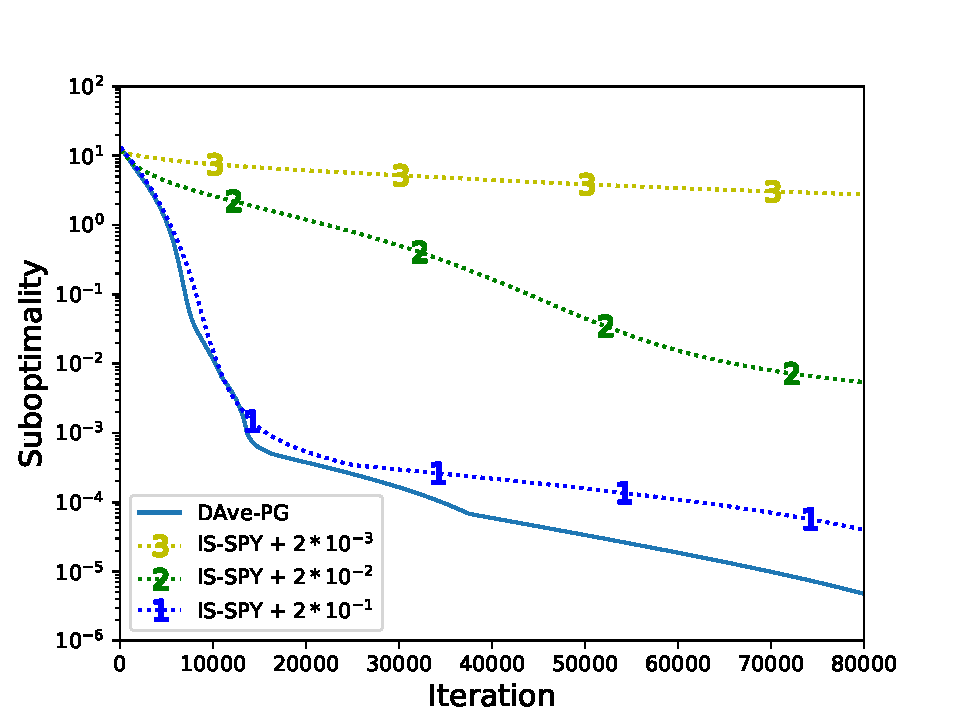
\includegraphics[width = 0.49\linewidth]{distributed/figs/madelon_10w_001_0001_fun_vs_ite_log_coordinate_stupid.pdf}}
 \hfill
\subfloat[][The functional suboptimality versus amount of coordinates sent during communication rounds.]{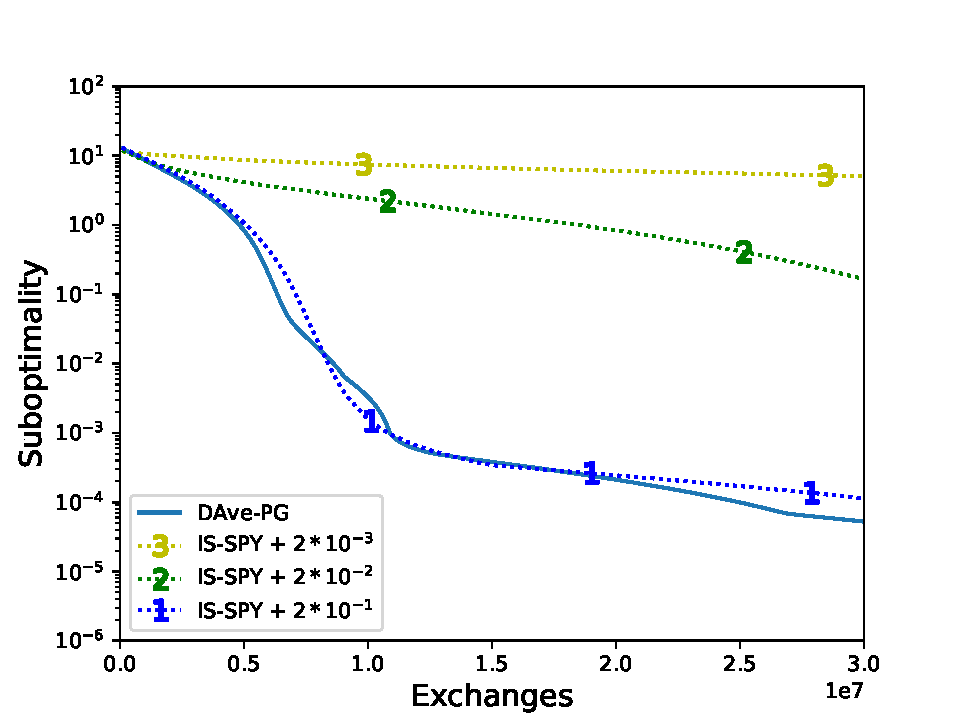
\includegraphics[width = 0.49\linewidth]{distributed/figs/madelon_10w_001_0001_fun_vs_ex_log_coordinate_stupid.pdf}}
\end{center}
\caption{Evolution of \maskalgo~iterates comparing to \dave. We consider logistic regression objective function with elastic net regularizer on Madelon dataset from LibSVM library \cite{chang2011libsvm}. We denote by ``SPY-DR~+ $p$'' the \maskalgo with selected as in Option I of Assumption \ref{hyp:algoident} with probability $\pi = p$.}
\label{fig:spydr}
\end{figure}

\section{Conclusion}
In this chapter, we present the idea of sparsification of \dave~algorithm and showed that in case of uniform or ``scaled-adaptive'' sampling algorithm converges almost surely to the minimizer and as a result identifies the near-optimal sparsity structure of the solution. However, both in theory and in practice, the convergence of sparsified algorithm is worse than without sparsification that requires further development. First, in Chapter XXX, we propose the reconditioned version of the \salgo with adaptive sampling that could overcome both issues: non i.i.d. of the sparsity mask selectors and ill-conditioned problems. Second, in Chapter YYY we investigate the empirical performance of \salgo with adaptive selection to see if it performs well in practice.
}